\chapter{System Design}
This section is concerned with how the application was made, with in-depth detail on the FrontEnd, BackEnd, architecture, deployment, how these features were made, and designed.

\section{Architecture}
The below figure \ref{image:Architecture} shows a system diagram overview architecture of the application
\begin{figure}[h!]
    \centering
    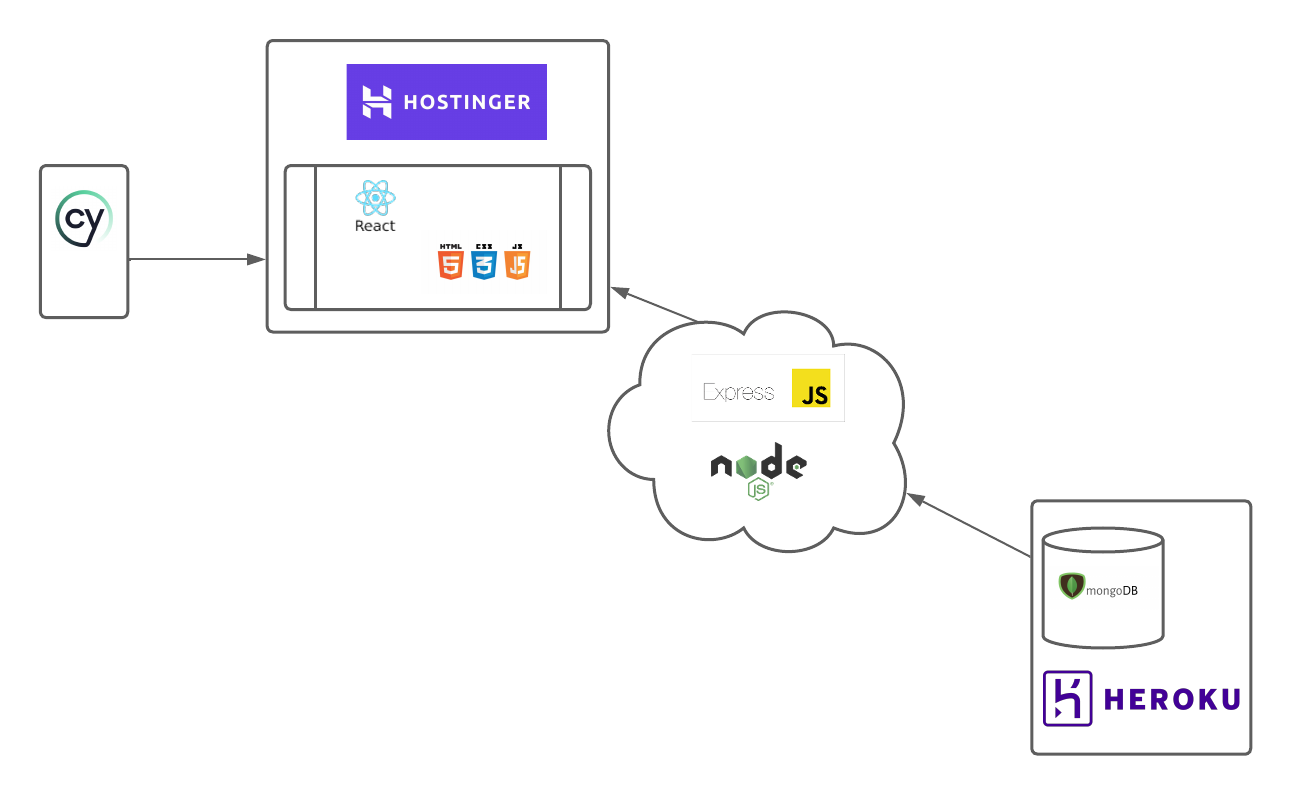
\includegraphics[width=0.8\textwidth]{images/SystemDiagram.png}
    \caption{System Architecture}
    \label{image:Architecture}
\end{figure}

\section{Front End Component Tree }
The below figure \ref{image:ReactTree} shows a high level tree of the various components in the front end of the application.
\begin{figure}[h!]
    \centering
    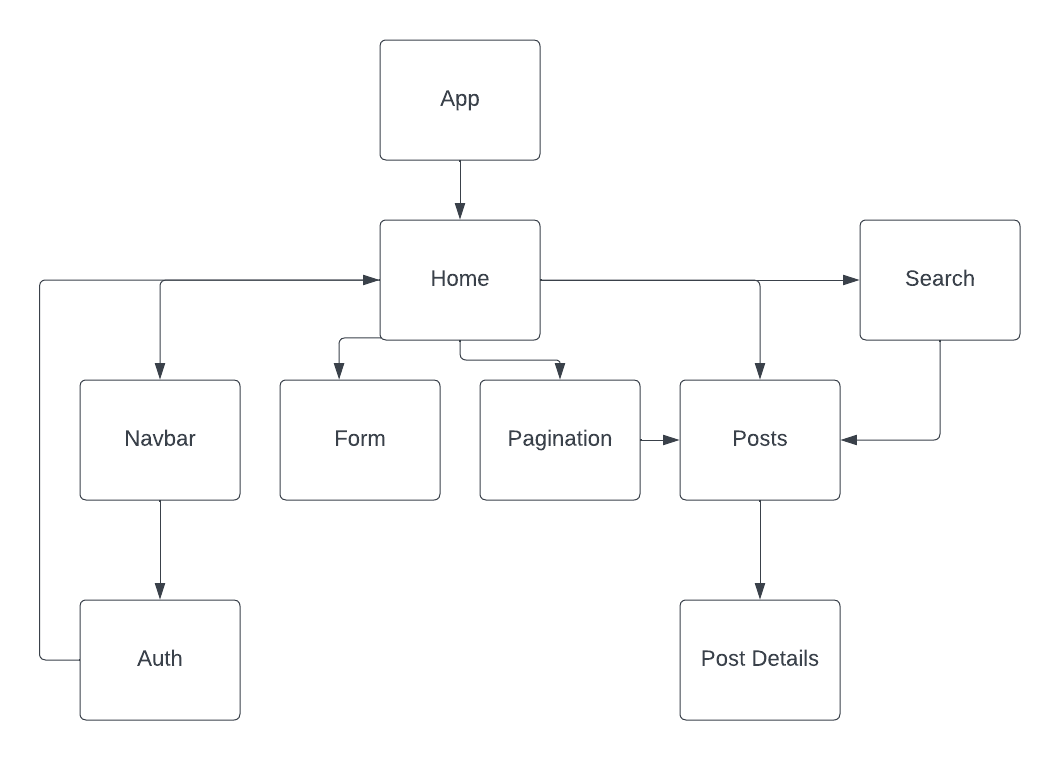
\includegraphics[width=0.8\textwidth]{images/ReactCompTree.png}
    \caption{React Component Tree}
    \label{image:ReactTree}
\end{figure}

\section{Front End Home}
The home page react component of the application encompasses rendering the home page, along with creating and viewing posts, lastly the home page is concerned with searching for a particular post.
\begin{figure}[h!]
    \centering
    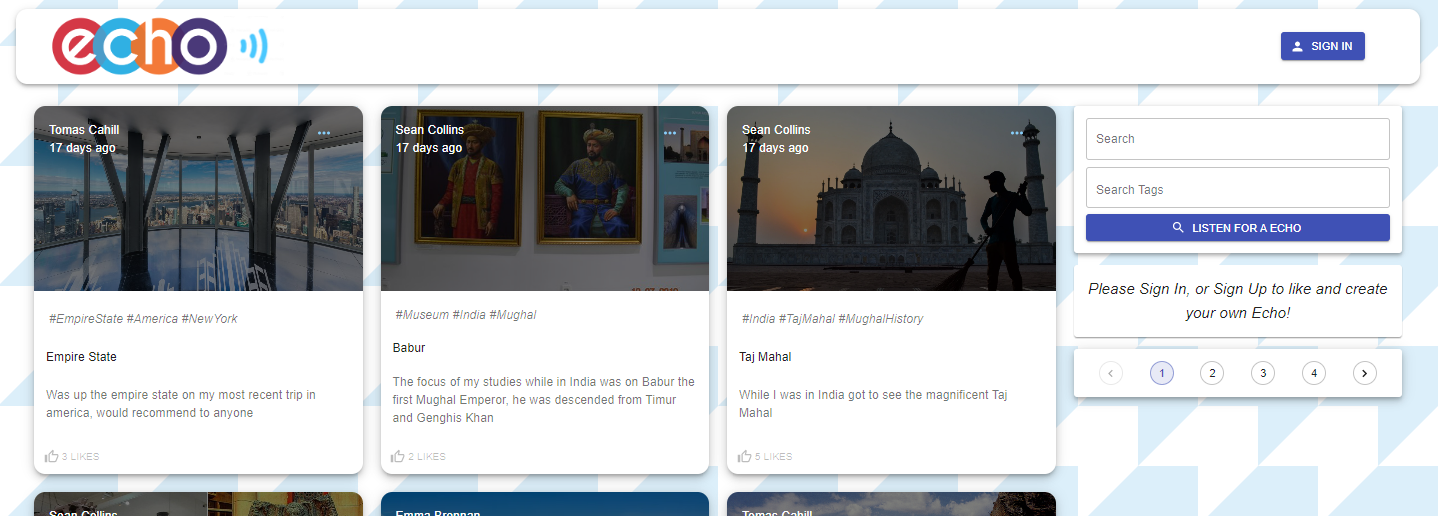
\includegraphics[width=0.7\textwidth]{images/HomePage.png}
    \caption{Home Page}
    \label{image:HomePage}
\end{figure}

\subsection{Rendering Home Page}
The home page renders various UI components such as Posts, Form, TextField, ChipInput, and Pagination using JSX syntax.  In addition it applies Material UI styles to these components using the useStyles hook.
\subsection{Search}
Search uses the useState hook from react to store the search term, or if the user uses tags instead these are stored as an array of tags using useState, subsequently useDispatch is used when the user clicks on the search button updating the URL using history.push method then displaying the desired echo. The above mentioned, dynamically search's for specific tags or search bar term based on user inputs. The tags will only be inputted into the application when the user presses the enter button.
\begin{figure}[h!]
    \centering
    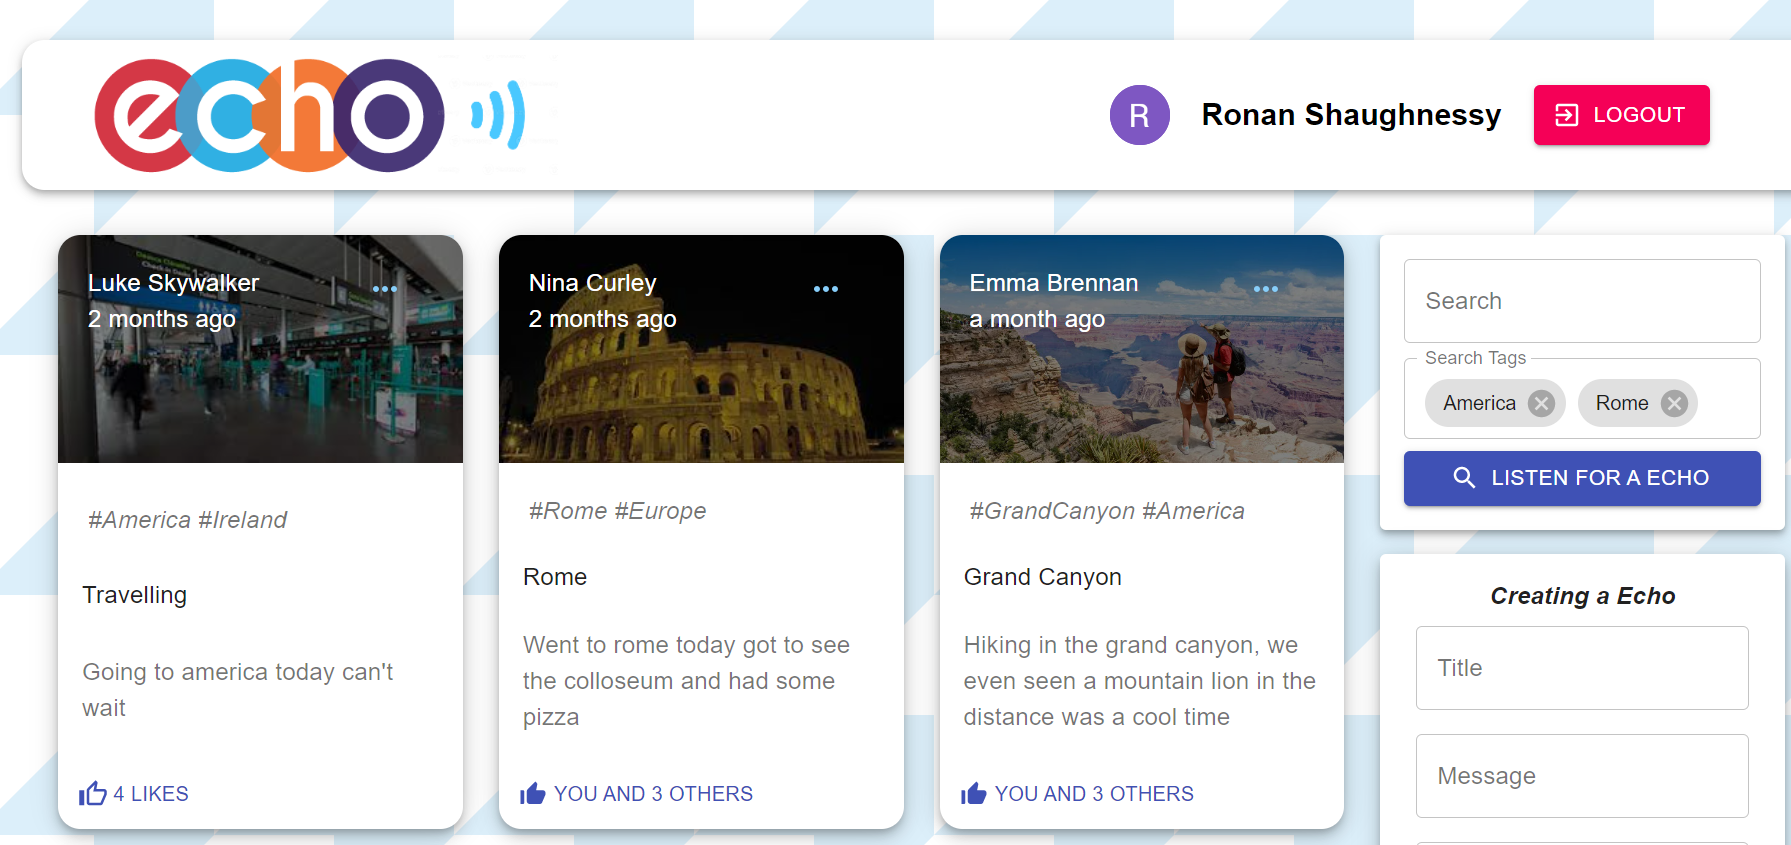
\includegraphics[width=0.7\textwidth]{images/SearchTags.png}
    \caption{Searching dynamically using tags}
    \label{image:SearchTags}
\end{figure}
\subsection{Viewing Posts}
The posts component is imported in order to view stored posts on the home page, setCurrentId is passed from posts allowing signed in users to be able to preform CRUD operations on a certain post. The setCurrentId function is defined using the useState hook. It updates the state of the currentId when the user selects a post to like or delete if applicable.

\subsection{Creating Posts}
Creating a post can be done on the home page using the form component in which the react useState is called. This hook is used to maintain its own local state for the form fields, including postData, which contains the data for the post being created. Then when the handleSubmit function is called by clicking the submit button, a createPost action uploads the new post with the data inputted in the form and adds it to the application state.

\section{Front End Form}
The form react component is responsible for creating a post once the user is signed in, the form component is imported into the home component to be rendered on the homepage.
\begin{figure}[h!]
    \centering
    \includegraphics[width=0.2\textwidth]{images/form.png}
    \caption{Form rendered on home page}
    \label{image:Form}
\end{figure}
\newline
The form only appears for a signed in user using JSON to parse local storage to see if a 'profile' is present, otherwise a message appears telling the user to sign in to create a echo. The currentID prop is used to see if the currentID is zero, if it is, then use dispatch to post the data through to the backend, when the relevant post details are filled out. Then the currentID prop is used to assign id's to the created posts, in which the id is assigned to the made post, and then  is used when a user wishes to see a post in more detail under the post details component.

\section{Front End Pagination}
The Pagination component is a simple component which allows to user to view posts on different pages by accepting a page parameter, then using the useSelector hook to access the number of pages of which this value is stored in redux. Next the useEffect hook dispatches the action getPosts, in order to recover the number of posts for the page, of which six are displayed on each page. The useEffect hook contains a page parameter to dynamically change every time the getPosts action is called, this is to facilitate posts being deleted or created.
\begin{figure}[h!]
    \centering
    \includegraphics[width=0.4\textwidth]{images/paginate.png}
    \caption{Pagination rendered on home page}
    \label{image:Paginate}
\end{figure}

\section{Front End Navbar}\label{section:navabr}
The navbar component is responsible for rendering the navbar and displaying it at the top of the application \ref{image:HomePage}. This component contains a button to sign in the user bringing the user to the auth route. When the user state is initialized using the useState hook, this parses a profile to assert if a user is signed in, then the navbar will display the signed in user and their avatar. Then when a user is signed in, the logout function can be used to dispatch a redux action to logout the user when the logout button is clicked, therein logging out the user. Finally when the user is signed in a JWT token is created, this token then expires after a specified amount of time automatically signing out the user with the useEffect hook.

\section{Front End Auth}
The auth component which can be sub typed into two forms which change if the user clicks the bottom button, launching the switchMode function to change the form to one of these options, sign in or sign up. Other functions such as the showPassword method is included, allowing the user to be able to click the eye button toggling the view of their password.

\subsection{Front End Sign Up}
Manually signing into the application can be done using the aforementioned bottom button and clicking it to switch the form, allowing the user to manually fill out their details. Error checking is preformed on this form to assert that the user cannot use an email that has already been picked, or if their passwords do not match.

\begin{figure}[h!]
    \centering
    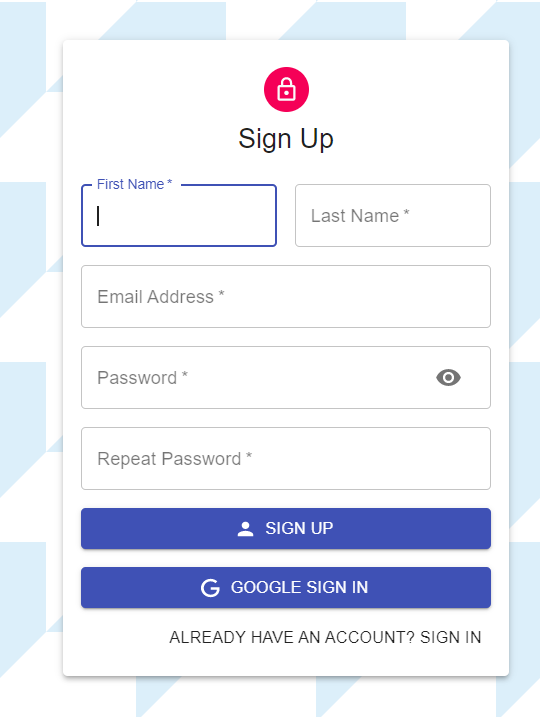
\includegraphics[width=0.5\textwidth]{images/SignUp.png}
    \caption{Sign Up Form}
    \label{image:SignUp}
\end{figure}

\newpage
\subsection{Front End Sign Up Verification Email}
Additional verification for when a user signs up to the application is used, as a welcome email appears when a user has signed up correctly. This email is sent using a BackEnd controller which can be seen here \ref{subsub:sendMail}. Below is the welcome the user receives following completion of signing up.
\begin{figure}[h!]
    \centering
    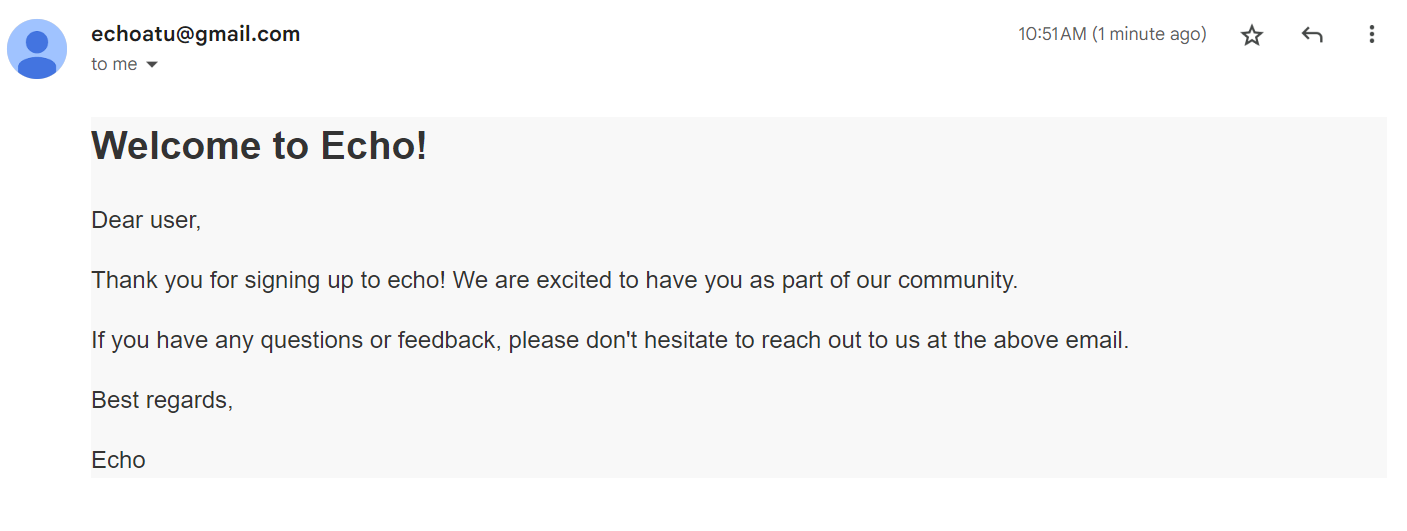
\includegraphics[width=0.5\textwidth]{images/WelcomeEmail.png}
    \caption{Welcome email user receives}
    \label{image:WelcomeEmail}
\end{figure}

\subsection{Front End Sign In}
A user can sign into the application in two ways, one is done manually when the user signs up, filling out their details. The users data is then stored into a object called formData, this data is relayed to the backend where it is stored in the database allowing the user to sign in later. The Second option for a user to sign in is using the GoogleLogin component from react-google-login, wherein a useEffect hook is called to load the Google API client library and initialize it with the client ID, thereby signing in the user without having to manually fill out their details, this is assuming the user has a google account.

\begin{figure}[h!]
    \centering
    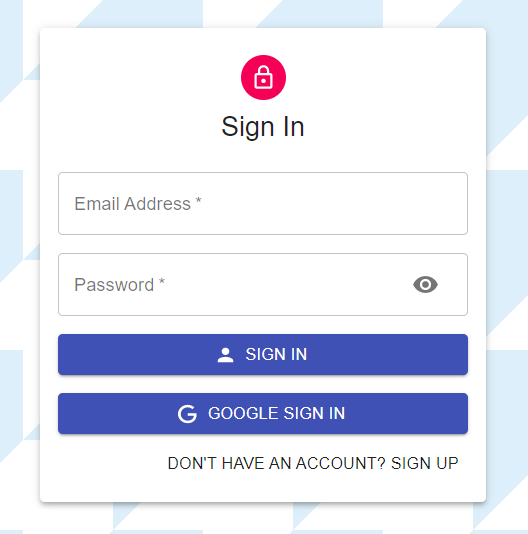
\includegraphics[width=0.5\textwidth]{images/SignIn.png}
    \caption{Sign In Form}
    \label{image:SignUp}
\end{figure}

\section{Front End Posts}
This react component manages rendering posts that the user makes in the form component as can be seen from this figure \ref{image:HomePage}. Posts lends to the search logic as there is a if statement, stating if the user has searched and no such post exists then a warning message appears. If there are posts to display to the user, a map function is called to iterate over each post and displays each of the Post components which meet the search parameters.

\subsection{Front End Post}
Inside the posts component is a sub component called post that is in control of rendering each single post and their associated content which is pulled from the database. Assuming the user is signed in, functions such as liking and deleting posts will appear for the user. These actions are controlled by using, useDispatch to make a call to redux actions to handle the like, and deleting functions. The user can also click the ellipses on the top right to view a single post in more detail.

\section{Front End Post Details}
Post details provides an in depth look at a single post, using the useSelector hook provided by react-redux library to get the state data, then rendering the aforementioned data using conditional statements. Dispatch is used to call the getPost method that gets an id parameter to fetch the particular post the user has selected from the server. Posts with similar tags will be displayed on the bottom of the page, these posts are stored as a array of recommendedPosts, which are found by filtering posts in the redux store to exclude unrelated posts, based on their tags. These recommended posts can be clicked, then using the history object from react-router-dom to route to the selected post.
\begin{figure}[h!]
    \centering
    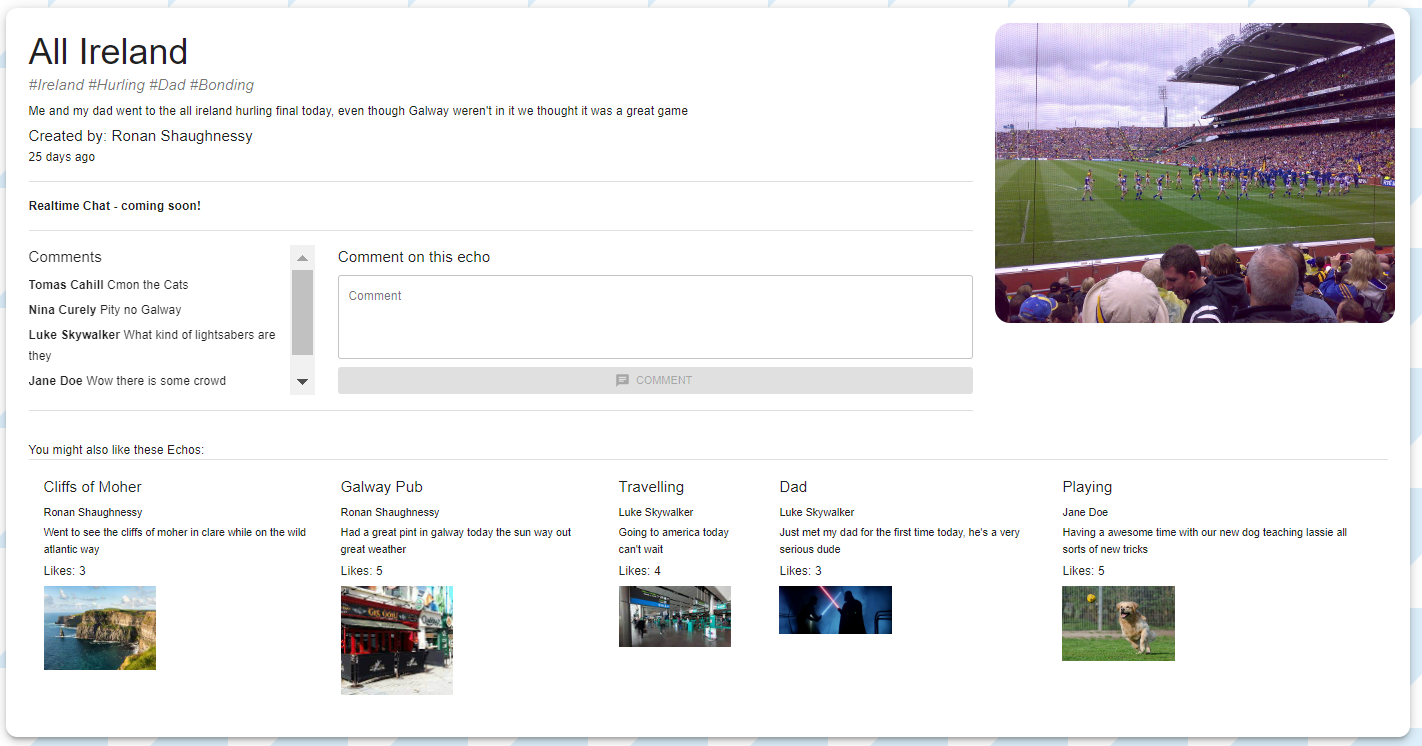
\includegraphics[width=0.5\textwidth]{images/PageDetails.png}
    \caption{Page Details}
    \label{image:PageDetails}
\end{figure}
\section{Front End Post Details Comment Section}
The comment section of the page details component is a sub component, the page details imports the comments section and renders it on the left side of the page details as seen in figure \ref{image:PageDetails}. React hooks such as useState are used to mange the comment state wherein comments are initially set to false provided there is no comments. A function called handleComment is called when the user types in a comment into the input box and clicking the comment button. This function gets the user name from local storage so their name will appear next to the comment, then using redux to dispatch an action adding the new comment to the database, finally updating the comment state with the new comment clearing the old input.

\section{Miscellaneous Front End Post Features}
Feature which don't fall into any particular category in terms of high or low level design.

\subsection{Circular Progress Bar}
If internet access is not very fast where a user is accessing the application, a circular progress bar will appear so as the user is aware that the application is loading, and that the application has not crashed.

\subsection{Kommunicate Bot}
If a user is having difficulty using the program, an AI chat bot system has been set up to answer various inquiries if the user is lost or unclear how to perform something on the site.
This was added into the indes.html file, with code provided by kommunicate to call an API which I set up containing the specifically configured bot for this application.

\section{Back End}
The back end of the application is a node.js server using express as a framework, then accessing the mongoDB database using mongoose to listen on the specified port.

\section{Back End Model View Controller}
The Model View Controller below \ref{image:MVC}, shows a high-level diagram of how the back end interacts with the application in general, where it relays information the user passes into the application, either submitting a response or adding information to the application.
\begin{figure}[h!]
    \centering
    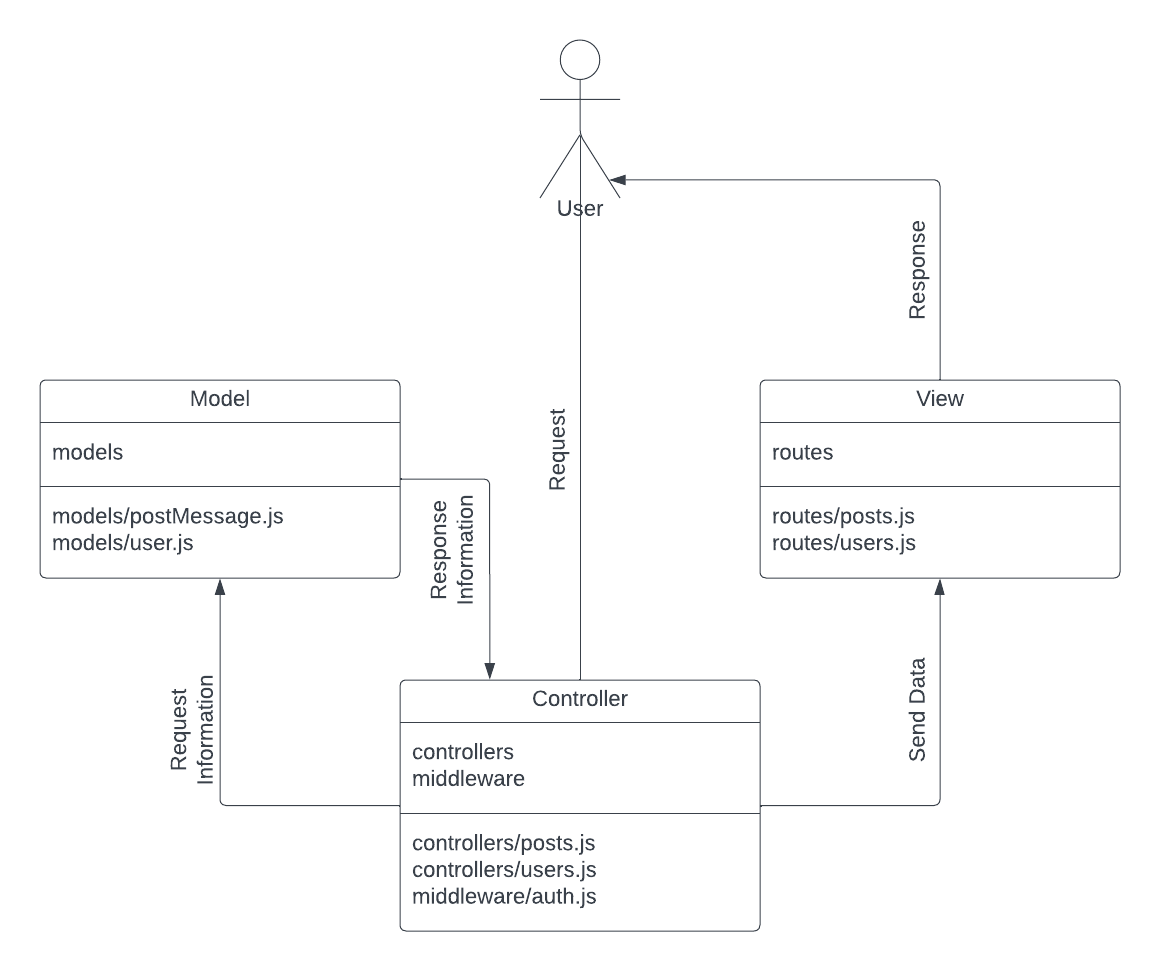
\includegraphics[width=0.8\textwidth]{images/MVC Diagram.png}
    \caption{Model View Controller Diagram}
    \label{image:MVC}
\end{figure}

\newpage
\section{Back End Controllers}
Two modules which interact as controllers for the application are the middleware, and the controllers folder modules.
\begin{figure}[h!]
    \centering
    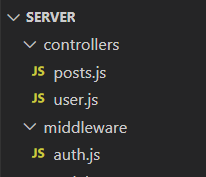
\includegraphics[width=0.2\textwidth]{images/Controllers.png}
    \caption{Controllers present in file system}
    \label{image:Controllers}
\end{figure}

\subsection{Back End post.js controller}
The post.js controller handles all routes except for the authorization routes. A router object is created at the top of the script, this allows the routes to be used in the front end of the application. A number of functions are declared in the script, for example the createPost function in which will briefly be described. The aforementioned function creates a new post with the data the user sends to the back end in the request body, wherein the function then adds the users ID, time the post was committed, and saves it to the database. A status code will then be sent to the front end of 201 for a successful request response, or 409 if there is an error. The above-stated code can be view below \ref{image:createPost}.
\begin{figure}[h!]
    \centering
    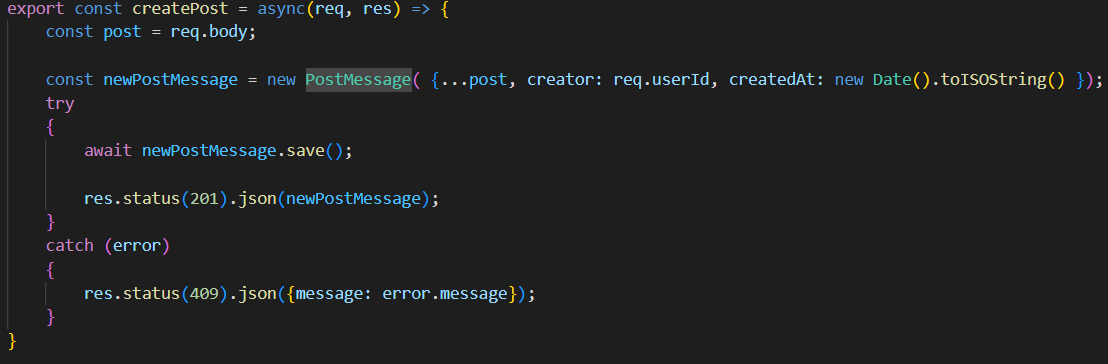
\includegraphics[width=0.8\textwidth]{images/createPost.png}
    \caption{Controller, creating a post}
    \label{image:createPost}
\end{figure}

\subsection{Back End user.js controller}
The user controller interacts in a similar way to the post controller, except in that the user controller is used as part of the authorization level of the application. Imported for this script is jsonwebtoken which is used to generate a JSON web token for authentication.
\begin{figure}[h!]
    \centering
    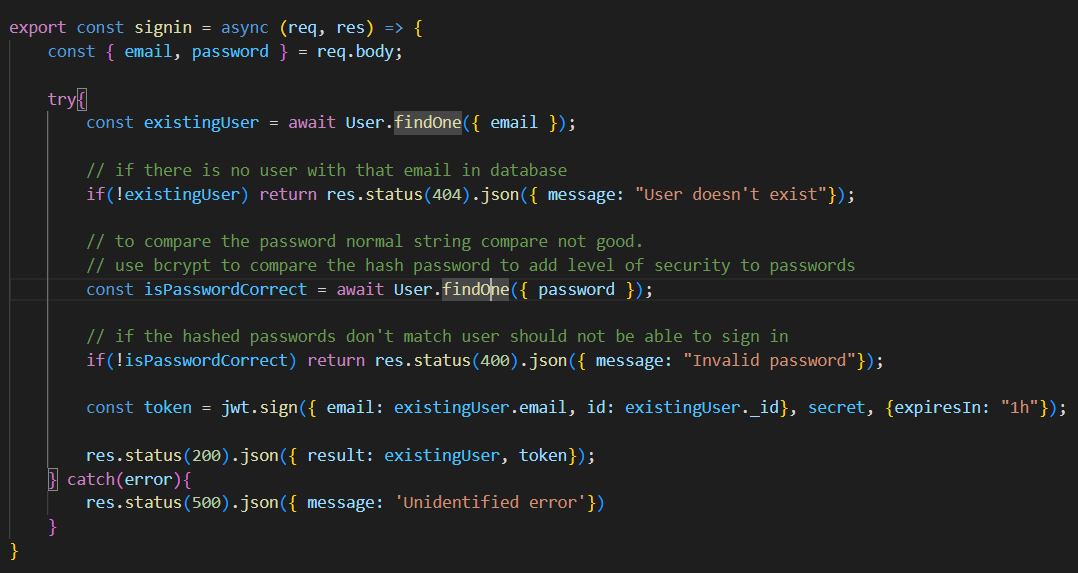
\includegraphics[width=0.8\textwidth]{images/signInCode.png}
    \caption{Controller, signing in a user}
    \label{image:signInCode}
\end{figure}
\newline
The above figure \ref{image:signInCode}, illustrates from a internal view, the programming involved in creating authorization manually. In the above function signin handles logic related to logging in. Firstly, the function pulls out the email and password the user has submitted from the request body, checking against the database using the User.findOne method to assert the email exists. If no email matches, a 404 error is returned. Secondly using the same logic as before to assert if the passwords match, if not then an error status of 400 is returned. If the password and email match, a JSON web token is created which contains the users ID and email thereby signing the user in, sending a status code of 200. The JSON web token is then configured to expire in one hour, after which the user will have to sign in again.

\subsubsection{Back End sendEmail}\label{subsub:sendMail}
The logic for sending an email from Echo's admin email to a newly registered user is handled in the function block below. The aforementioned is accomplished through the use of nodemailer library methods such as createTransport, which creates an object for sending the email i.e who it is sent by, mailOptions, which defines the details of the email to be sent, and finally sendMail, which sends the email with the prior methods filling out the details. This function is then called in the signup function block, passing in the email the user has signed up with providing it is a actual email.
\begin{figure}[h!]
    \centering
    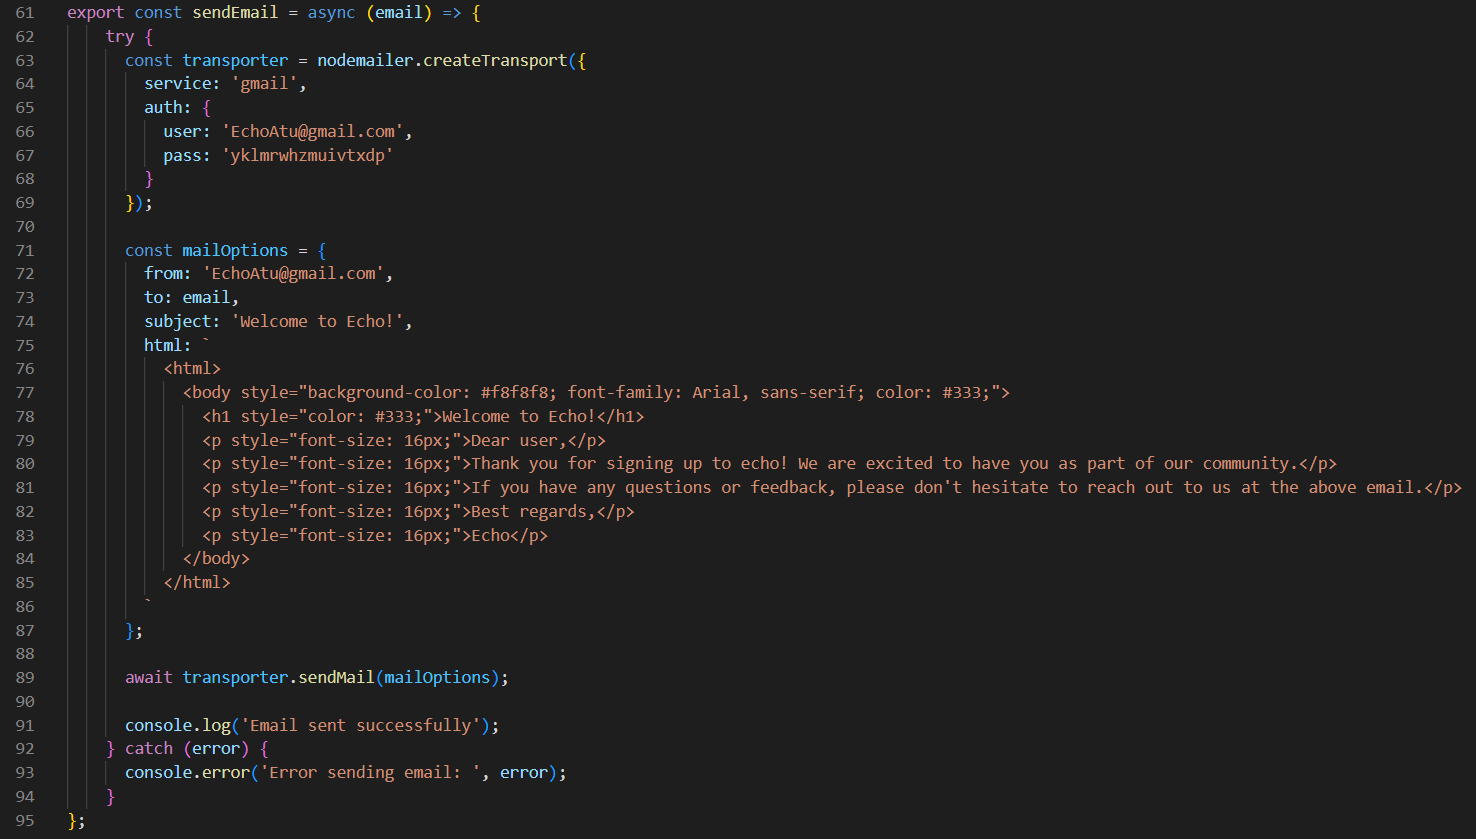
\includegraphics[width=0.5\textwidth]{images/sendEmailController.png}
    \caption{Logic to send an email to signed up user}
    \label{image:sendEmailController}
\end{figure}

\subsection{Back End auth.js middleware}
The middleware interacts with the controllers to provide an extra layer of authorization to the application, thereby passing in the middleware to the user controller, then certain functions for example liking are only available to those who sign in or up to the application. The middleware uses the jwt.verify method to assert the custom token then setting the userID property of the req object to the id property of the decoded token. If it is not a custom token the function decodes the token using the decode method and sets the userId property of the req object to the sub property of the decoded token. Lastly next is called to pass control to the user.js file in the controllers folder.

\begin{figure}[h!]
    \centering
    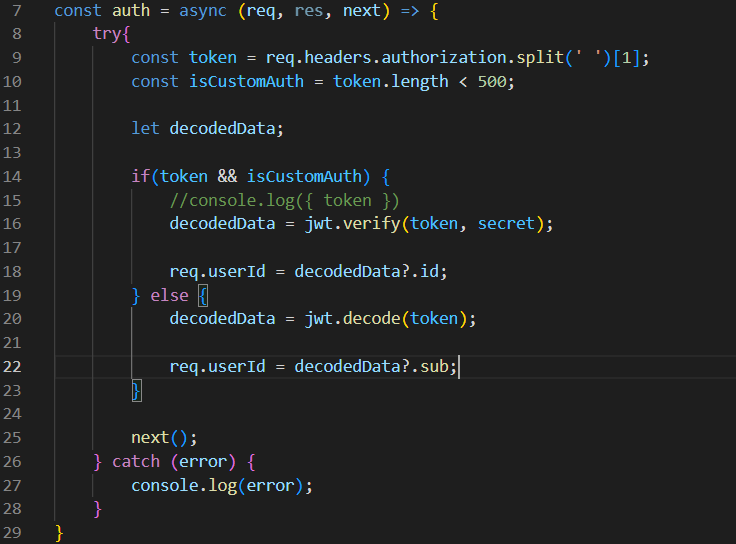
\includegraphics[width=0.5\textwidth]{images/BackEndMiddle.png}
    \caption{Logic in the auth.js middleware}
    \label{image:BackEndMiddle}
\end{figure}

\section{Back End Models}
As shown below, Mongoose is used to implement two schema that are used in the application. The schema is used when performing various CRUD operations. First and foremost, the schema function accepts various objects with a schema definition in order to establish the schema. Second, mongoose.model is used to create the collection in the database, with the collection name as the first argument and the schema as the second.
\begin{figure}[ht]
\begin{minipage}[b]{0.4\linewidth}
    \centering
    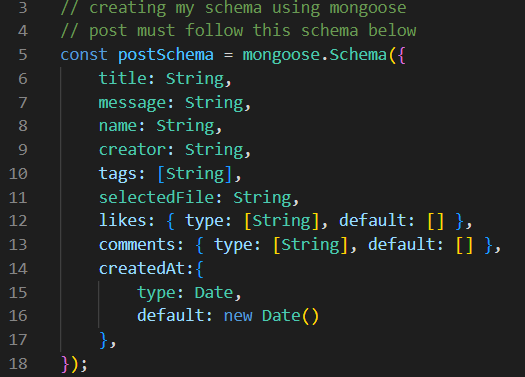
\includegraphics[width=\linewidth]{images/postMessageModel}
    \caption{Post Message Model}
\end{minipage}
    \hspace{0.5cm}
    \begin{minipage}[b]{0.5\linewidth}
    \centering
   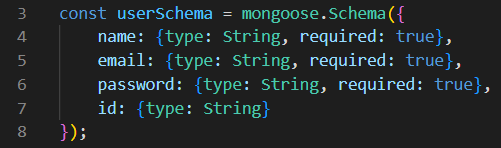
\includegraphics[width=\linewidth]{images/userModel}
    \caption{User Model}
\end{minipage}
\end{figure}

\subsection{User Model}
As previously stated, mongoose is imported into the script, and then the schema is initialized. The user must then follow the predefined schema in order to be saved properly in the database. This model in particular, is only concerned with the user signing in or up, as such the fields in this model are id, name, email, password, all of which a required fields except for id.
\subsection{Post Message Model}
Similarly to the previous model with some noticeable changes, the postMessage schema has more objects such as title, message, creator, tags, name, and selectedFile. Likes, comments, and createdAt are three distinct objects in the schema. Likes are an array of strings that are set to default, so that no post will have any likes when it is posted until a user actively likes it, at which point the like will be saved in the database. Comments work similarly to likes in that none appear in the database until a user leaves a comment on a post. Finally, the other distinct object createdAt has a field type, and date. When a user posts their echo, the default: new Date() function is used to give the exact date the post was made at, e.g. if the was made an hour ago, it will say thus, and so on.

\section{Back End Routes}
This section is concerned with the application's routes and the view section of the model view controller. The implemented scripts make use of express to handle the application's HTTP requests. The routes receive data from the controllers, then sending it to the user in a response. The majority of HTTP requests sent to the front end are get, post, patch, and delete.
\begin{figure}[ht]
\begin{minipage}[b]{0.4\linewidth}
    \centering
    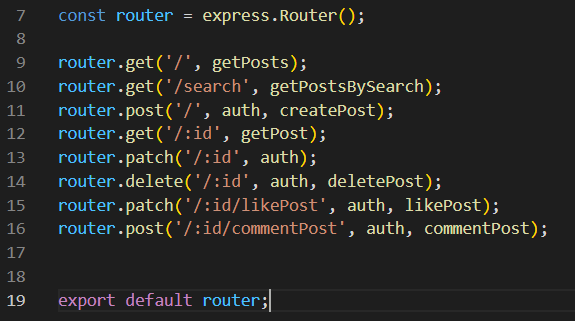
\includegraphics[width=\linewidth]{images/routePosts}
    \caption{Posts.js Routes}
\end{minipage}
    \hspace{0.5cm}
    \begin{minipage}[b]{0.5\linewidth}
    \centering
   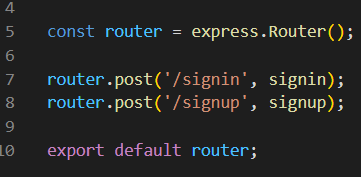
\includegraphics[width=\linewidth]{images/routeUsers}
    \caption{Users.js Routes}
\end{minipage}
\end{figure}

\subsection{Posts.js}
The applications most common response from the routing is the router.get('/', getPosts), this route handles GET requests, calls the getPosts function to retrieve a list of all posts as seen in \ref{image:HomePage}. Second, router.post('/', auth, createPost) handles a post request to the URL, requiring middleware authentication, if the authentication is successful, the user can call the createPost function from the controller. Finally, delete('/:id', auth, deletePost) handles a delete request on a specific post, asserting that the specific user has the correct id to be able to delete the post they wish to remove, this route also requires authentication.

\subsection{Users.js}
Two routing methods are present in this script strictly relating to authentication, both being HTTP post methods. Firstly router.post('/signin', signin) handles the user signing into the application, then calling the signin function from the controller, this route is used to assert the credentials through the controller. Next router.post('/signup', signup) handles the user signing up to the application, then using the signup function in the controllers to create a new user with the provided credentials

\section{Deployment}
The final phase of the the design was to deploy the application onto the internet, this was done with two hosting sites, hostinger and heroku.

\subsection{Heroku}
The server side was deployed to heroku using the heroku CLI, then the package.json script for the server was changed from start: nodemon to start:"node index.js" which makes it easier to run as npm run start is no longer required every time, and the server does not need to be run locally anymore, now there can exist two environments, so as there is always a stable version of the server online. Secondly the index script was changed to give an alert message to assert the server side is running.
\begin{figure}[h!]
    \centering
    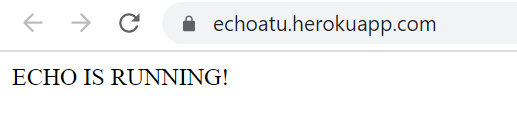
\includegraphics[width=0.5\textwidth]{images/deployment.png}
    \caption{Heroku Deployment}
    \label{image:deployment}
\end{figure}
\subsection{Hostinger}
In order to link the server to the client, the below code was changed from localhost:5000, to the deployed heroku url.
\begin{figure}[h!]
    \centering
    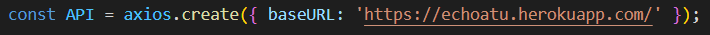
\includegraphics[width=0.5\textwidth]{images/herokuDeploy.png}
    \caption{Connection of server to client}
    \label{image:herokuDeploy}
\end{figure}
After that, using the node command npm run build to build the client side. SSL \cite{hickman1995ssl} must be installed on hostinger, which provides the application with https security. Finally, once the application has completed the npm run build command, the build files must be dragged into the file manager on hostinger, and hostinger will build the clientside of the application, so that it can be accessed using the domain name specified when creating a website on hostinger. The application can then be seen on echoatu.com \ref{image:HomePage}.